\documentclass{beamer}

\title{The Impact of Anthropogenic Forcing on ENSO Amplitude}
\author{Ben Goldman}
\date{\today}

\usepackage{natbib}
\usepackage{tikz}
\usepackage{varwidth}
\usepackage{hyperref}
\usepackage[orientation=landscape, size = a4 , scale=1]{beamerposter}
\usepackage{lipsum}

\usetikzlibrary{arrows,backgrounds}
\usetikzlibrary{positioning}
\tikzstyle{process}=[rectangle, draw=process, fill=process!20, line width = 0.3mm]
\tikzstyle{data}=[rectangle, draw=data, fill=data!20, line width = 0.3mm]
\tikzstyle{tight}=[node distance = 0.5in]
\tikzstyle{loose}=[node distance = 2in]
\definecolor{process}{HTML}{3d5f8f}
\definecolor{data}{HTML}{8f6d3d}

\usetheme{ben}

\newcommand{\myfig}[4]{
\begin{figure}
  \centering
  \includegraphics[width=#3\textwidth]{figures/#1}
  \caption{#2}
  \label{fig:#4}
\end{figure}
}

\graphicspath{{./figures}}

\renewcommand{\bibsection}{}

\begin{document}

\begin{frame}
  \begin{columns}
    \column{.333\textwidth}
    \begin{block}{}
        \bf\huge{Conclusion/Application}
        \vspace{5in}
        \bf\huge{Future Research}
    \end{block}
    \column{.333\textwidth}
    \begin{block}{Back Panel}
    \end{block}
    \column{.333\textwidth}
    \begin{block}{}
      \begin{center}
        \bf\huge{The Impact of Anthropogenic Forcing on ENSO Amplitude}
      \end{center}
      \begin{figure}
        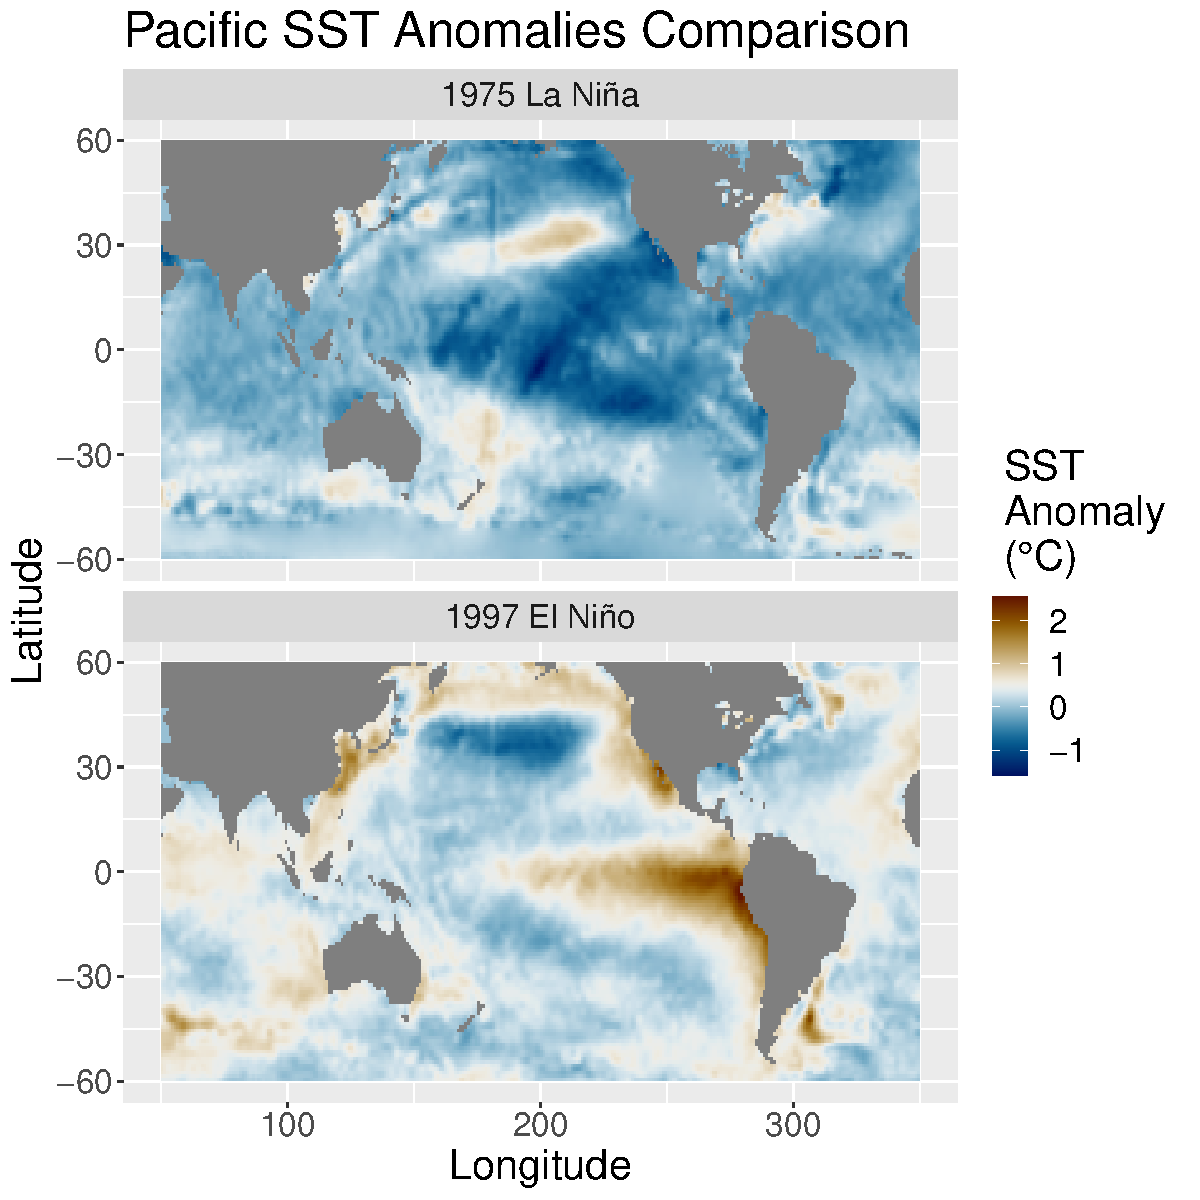
\includegraphics[width=\textwidth]{intro_fig}
      \end{figure}
    \end{block}
  \end{columns}
\end{frame}

\begin{frame}
  \begin{columns}
    \column{.333\textwidth}
    \begin{block}{Introduction}
    \end{block}
    \begin{block}{Problem Statement}
    \end{block}
    \column{.333\textwidth}
    \begin{block}{Goals}
    \end{block}
    \begin{block}{Methodology}
    \end{block}
    \column{.333\textwidth}
    \begin{block}{Results/Discussion}
    \end{block}
  \end{columns}
\end{frame}

\end{document}
